% \documentclass[12pt, twoside]{article}
\usepackage[letterpaper, margin=1in, headsep=0.2in]{geometry}
\setlength{\headheight}{0.6in}
%\usepackage[english]{babel}
\usepackage[utf8]{inputenc}
\usepackage{microtype}
\usepackage{amsmath}
\usepackage{amssymb}
%\usepackage{amsfonts}
\usepackage[nomessages]{fp} %\FPeval{\var-name}{2*sin(pi/6)}
\usepackage{siunitx} %units in math. eg 20\milli\meter
\usepackage{yhmath} % for arcs, overparenth command
\usepackage{tikz} %graphics
\usetikzlibrary{quotes, angles, arrows, arrows.meta}
\usepackage{graphicx} %consider setting \graphicspath{{images/}}
\usepackage{parskip} %no paragraph indent
\usepackage{enumitem}
\usepackage{multicol}
\usepackage{venndiagram}

\usepackage{fancyhdr}
\pagestyle{fancy}
\fancyhf{}
\renewcommand{\headrulewidth}{0pt} % disable the underline of the header
\raggedbottom
\hfuzz=2mm %suppresses overfull box warnings

\usepackage{hyperref}

\fancyhead[LE]{\thepage}
\fancyhead[RO]{\thepage \\ Name: \hspace{4cm} \,\\}
\fancyhead[LO]{BECA / Dr. Huson / Geometry\\*  Unit 9: Dilation \\* 17 January 2022}

\begin{document}

\subsubsection*{9.1 Classwork: Dilation \hfill CCSS.HSG.SRT.B.5}
\begin{enumerate}
    \item Do Now: Plot and label the triangle $A'B'C'$. $A'(0,0)$, $B'(8,0)$, $C'(8,4)$.\\
    Make a list of comparisons of the two triangles: their sides' lengths, location, their angles, orientation, area and perimeter. \\
      \begin{tikzpicture}[scale=.7]
        \draw [help lines] (-1,-2) grid (9,6);
        \draw [thick, ->] (-1.2,0) -- (9.4,0) node [below right] {$x$};
        \draw [thick, ->] (0,-2.2)--(0,6.4) node [left] {$y$};
        \draw [thick] (0,0)node[below right]{$A$}--
         (4,0)node[below]{$B$}--
           (4,2)node[above left]{$C$}--cycle;
      \end{tikzpicture}
     \vspace{3cm}
  
\begin{multicols}{2}
[\item Find the missing angle measures. Are $\triangle CAT$ and $\triangle DOG$ congruent?] \vspace{0.5cm}
    \begin{tikzpicture}[scale=0.9]
      \coordinate [label=above left:$C$](A) at (95:2);
      \coordinate [label=below:$A$](B) at (0, 0);
      \coordinate [label=right:$T$](C) at (-10:3.5);
      \draw [thick] (A)--(B)--(C)--cycle;
      \draw [thick, xshift=3cm, yshift=1.5cm, scale=1.5] (95:2) node[above]{$D$}--
      (0,0) node[below]{$O$}--
      (-10:3.5) node[right]{$G$}--cycle;
    \end{tikzpicture}\\
    \begin{enumerate}
      \item $m\angle C =45^\circ$, $m\angle A =105^\circ$\\[0.25cm]
      .\hspace{1cm} $m\angle T =$ \rule{2cm}{0.15mm}
      \item $m\angle G =30^\circ$, $m\angle O =105^\circ$\\[0.5cm]
      .\hspace{1cm} $m\angle D =$ \rule{2cm}{0.15mm}
    \end{enumerate}
  \end{multicols}  \vspace{1cm}
      
\item This is the symbol for similar triangles: $\triangle ABC \sim \triangle DEF$. Write down two definitions of similar triangles.
  
\newpage
\item \begin{enumerate}
  \item Graph and label $\triangle ABC$ with $A(0,0)$, $B(3,2)$, and $C(3,0)$.
  \begin{center}
    \begin{tikzpicture}%[scale=.635]
      \draw [help lines] (0,0) grid (10,6);
      \draw [thick, ->] (0,0) -- (10.4,0) node [below right] {$x$};
      \draw [thick, ->] (0,0)--(0,6.4) node [left] {$y$};
    \end{tikzpicture}
  \end{center}
  \item Dilate or stretch the triangle by a factor of $k=3$ centered at the origin.\\ $\triangle ABC \rightarrow \triangle A'B'C'$
  \item Find each ratio or fraction. \\[0.5cm]
    $\displaystyle \frac{A'C'}{AC}=$ \hfill
    $\displaystyle \frac{B'C'}{BC}=$ \hfill
    $\displaystyle \frac{A'B'}{AB}=$ \hspace{2cm}
\vspace{1cm}
\end{enumerate}
\item Triangle $ABC$ is dilated with a scale factor of $k=\frac{5}{3}$ centered at $A$, yielding $\triangle ADE$, as shown. Given $AB=9$, $BC=12$, and $AC=15$. \\[0.25cm] Find $AD$, $AE$, and $DE$. \vspace{0.5cm}
   \begin{center}
       \begin{tikzpicture}[scale=0.4]
         \draw [thick]
         (0,0)node[left]{$B$}--
         (8,0)node[above right]{$C$}--
         (2,6)node[left]{$A$}--cycle;
         \draw [thick]
         (0,0)--
         (-1,-3)node[left]{$D$}--
         (11,-3)node[above right]{$E$}--(8,0);
         \node at (4,0)[below]{$12$};
         \node at (5.3, 3)[right]{$15$};
         \node at (0.3, 2.8)[above]{$9$};
       \end{tikzpicture}
     \end{center}

\newpage
Definition of \emph{similar} triangles: Triangles that have the same shape, but not necessarily the same size, are similar. Their corresponding angles are congruent and their corresponding sides are proportional. \\[1cm]
Dilation definition of similarity: Two figures are similar if one or more rigid motions and a dilation will carry one figure onto the other.

    

\end{enumerate}
\end{document}
